% !TeX root = ../main.tex
\section{问题二：基于严格因果预测与 CVaR 随机规划的日前购电策略}
\subsection{模型概述}
首先，采用季节朴素、岭回归和梯度提升树对负荷与光伏进行严格因果逐日预测，并基于近期历史残差生成整日场景。  
随后，建立带 CVaR 风险度量的两阶段随机线性规划模型，确定计划购电与储能调度，并控制预测偏差导致的高额紧急购电风险。  
此外，引入软终端项和年末 SOC 硬约束，保证储能调度的跨日平衡与全年连续性。

\subsection{符号说明}

问题二所用符号及其含义汇总于附录~\ref{app:q2_symbols}，正文各式中符号均在使用处给出定义。

\subsection{日前预测与联合场景构造}

\subsubsection{严格因果的日前预测}

为获得每日零时可用的负荷与光伏预测，本文建立历史时段中位数、岭回归与直方图梯度提升树三类候选模型。
在预测第 \(d\) 日时，首先使用截至第 \(d-2\) 日的数据训练候选模型，并根据第 \(d-1\) 日的加权绝对百分比误差（WAPE）选择最优模型。
最后使用截至第 \(d-1\) 日的全部历史数据重新训练该模型，得到第 \(d\) 日的点预测。

预测特征与选择指标 WAPE 的定义见附录~\ref{app:q2_calibration}。

正式报告期内，负荷预测的 MAE 和 WAPE 分别为
\(25.658\,\mathrm{kWh}\) 和 \(3.335\%\)，光伏预测的相应指标分别为
\(26.404\,\mathrm{kWh}\) 和 \(6.660\%\)。

\subsubsection{预测效果与负荷光伏联合场景构造}

点预测给出了负荷与光伏的日内变化趋势，但不能完整反映预测误差。在点预测基础上，采用整日残差块抽样生成负荷与光伏联合场景：
将当日负荷与光伏各144维预测残差合并为一个288维联合残差块；预测第 \(d\) 日时，从残差库中有放回地抽取历史日期 \(b_m\)，
并将同一日期的负荷与光伏残差同步叠加至对应点预测。第 \(m\) 个场景表示为
\begin{equation}
\begin{aligned}
    \boldsymbol{L}_d^{(m)}
    &=
    \max\left\{
    \boldsymbol{0},
    \widehat{\boldsymbol{L}}_d+
    \boldsymbol{\varepsilon}_{b_m}^{L}
    \right\},\\
    \boldsymbol{G}_d^{(m)}
    &=
    \max\left\{
    \boldsymbol{0},
    \widehat{\boldsymbol{G}}_d+
    \boldsymbol{\varepsilon}_{b_m}^{G}
    \right\},
    \qquad b_m<d
\end{aligned}
\label{eq:q2_joint_scenario}
\end{equation}

该做法可保留误差的日内变化特征，以及负荷误差与光伏误差之间的相关关系。
残差库按最近30个已结束日期滚动更新；不足30日时使用全部已有日期。
正式求解采用参数标定得到的 \(M=30\) 个场景。预测误差及联合场景的构造效果如图~\ref{fig:q2_prediction_scenario} 所示。

\begin{figure}[htbp]
    \centering

    \begin{subfigure}[t]{0.45\linewidth}
        \centering
        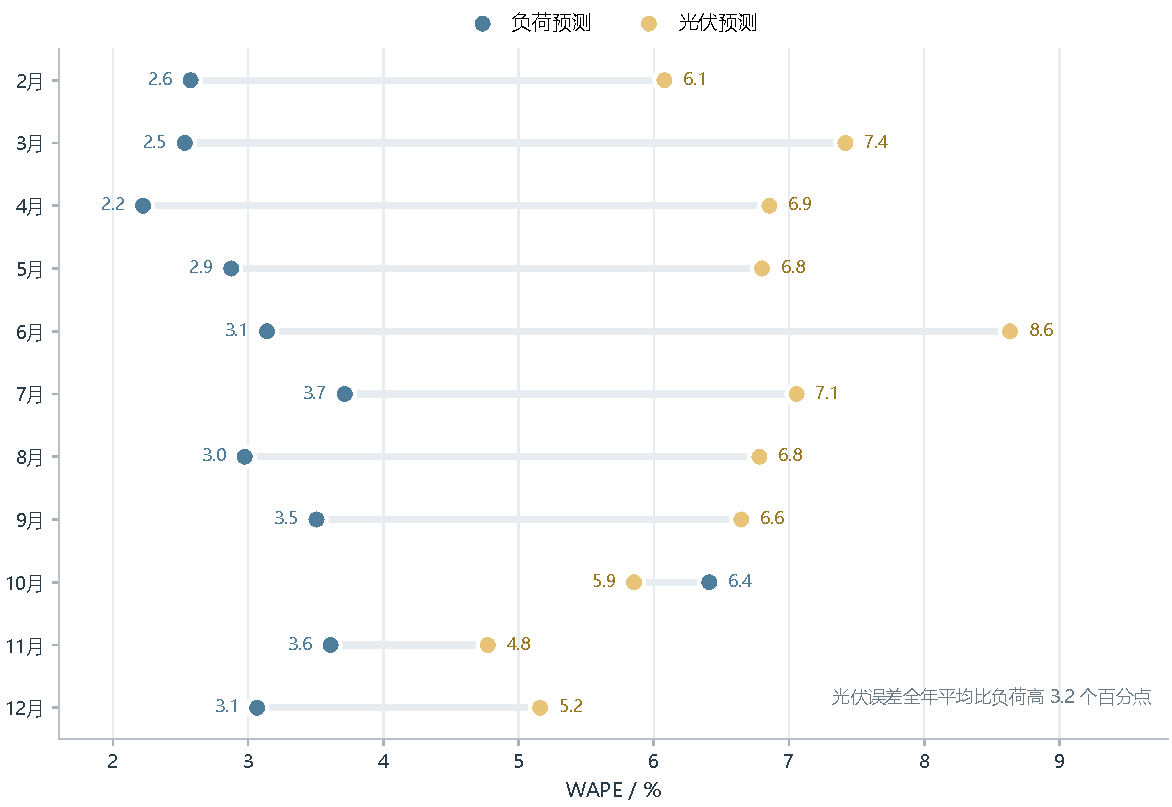
\includegraphics[width=\linewidth]
        {../All_Code/Q2_yy/Results/Pictures/fig_q2_error_monthly.pdf}
        \caption{负荷与光伏预测误差的月度变化}
        \label{fig:q2_monthly_error}
    \end{subfigure}
    \hfill
    \begin{subfigure}[t]{0.5\linewidth}
        \centering
        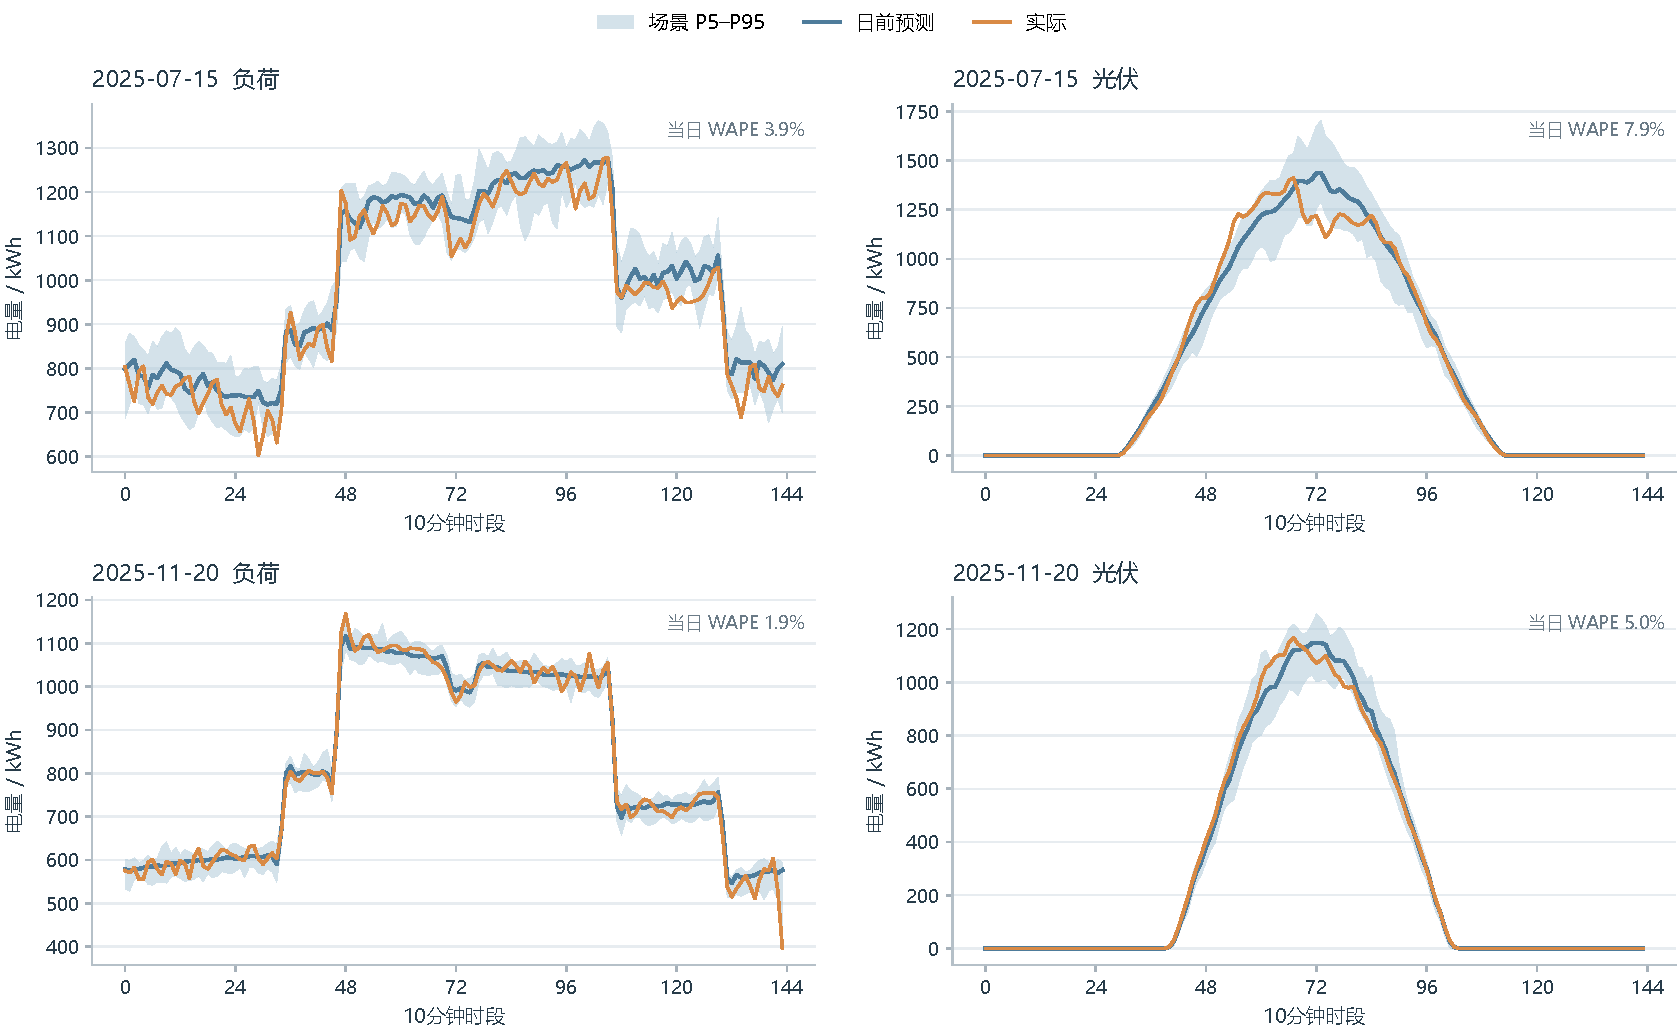
\includegraphics[width=\linewidth]
        {../All_Code/Q2_yy/Results/Pictures/fig_q2_load_pv_fan.pdf}
        \caption{代表日预测结果及场景分位区间}
        \label{fig:q2_load_pv_fan}
    \end{subfigure}

    \caption{负荷与光伏预测误差及联合场景构造结果}
    \label{fig:q2_prediction_scenario}
\end{figure}

由图~\ref{fig:q2_monthly_error} 可见，负荷与光伏预测的月度WAPE分别为
\(2.2\%\)至\(6.4\%\)与\(4.8\%\)至\(8.6\%\)，光伏较负荷高约3.2个百分点，
说明光伏出力具有更强的不确定性。

图~\ref{fig:q2_load_pv_fan} 中的阴影区域为场景集的\(5\%\)至\(95\%\)分位区间。
实际负荷与光伏曲线大部分位于区间附近，说明整日残差块抽样能覆盖点预测周围的主要波动。
\subsection{建立两阶段风险规避随机规划模型}

\subsubsection{目标函数}

根据前文生成的负荷与光伏场景，本文建立两阶段随机线性规划模型。
第一阶段在每日 \(0{:}00\) 确定计划购电量 \(x_t\)、计划充电量 \(c_t\)、计划放电量 \(r_t\) 和储电量 \(s_t\)，这些变量在全部场景中保持一致。
第二阶段根据各场景的负荷与光伏水平确定相应的调度决策。

由于计划购电按正常电价结算，紧急购电按同时段电价的5倍结算。
场景 \(m\) 下的购电费用为
\begin{equation}
    C_m
    =
    \sum_{t=1}^{T}\pi_t x_t
    +
    5\sum_{t=1}^{T}\pi_t e_t^m
    \label{eq:q2_scenario_cost}
\end{equation}

为兼顾平均购电费用与高费用场景风险，目标函数取期望费用与条件风险价值的加权组合：
\begin{equation}
\begin{aligned}
    \min J
    ={}&
    (1-\beta)\frac{1}{M}\sum_{m=1}^{M}C_m\\
    &+\beta\left[
    \zeta+
    \frac{1}{(1-\alpha)M}
    \sum_{m=1}^{M}q_m
    \right]\\
    &+\varepsilon\sum_{t=1}^{T}(c_t+r_t)
    +\kappa_2(\xi^++\xi^-)
\end{aligned}
\label{eq:q2_objective}
\end{equation}
其中，\(\alpha=0.90\)、\(\beta=0.20\) 分别为置信水平与风险权重，\(\zeta\) 为费用分布的风险阈值，\(q_m\) 为场景费用超出该阈值的部分。
正则项减少不必要的充放电循环，软终端项限制日末储电量偏离期初水平，两者均不计入实际购电费用。


\subsubsection{场景调度与储能约束}

场景实现后，日前购电量 \(x_t\) 已经确定，但允许部分电量不被提取。
设 \(y_t^m\) 和 \(u_t^m\) 分别为场景 \(m\) 下的计划电提取量和未提取量，\(g_t^m\) 和 \(w_t^m\) 分别为光伏利用量和弃光量，则
\begin{equation}
\begin{aligned}
    y_t^m+u_t^m &= x_t,
    &\qquad 0\leq y_t^m &\leq x_t,\\
    g_t^m+w_t^m &= G_t^m,
    &0\leq g_t^m &\leq G_t^m
\end{aligned}
\label{eq:q2_energy_allocation}
\end{equation}

电量分配后还需保证各场景的供需平衡。
充放电计划 \(c_t,r_t\) 在日前确定，场景实现后不变；可用电量不足时由紧急购电量 \(e_t^m\) 补足，固定放电产生多余供给时记为供给过剩弃电量 \(v_t^m\)。
各场景满足
\begin{equation}
    y_t^m+e_t^m+g_t^m+r_t
    =
    L_t^m+c_t+v_t^m
\label{eq:q2_scenario_balance}
\end{equation}
其中，\(e_t^m,v_t^m\geq0\)。

充放电计划在场景间一致，储能状态也由同一组计划决定。
考虑充放电损耗，储电量逐时段递推
\begin{equation}
    s_t
    =
    s_{t-1}
    +\eta_c c_t
    -\frac{r_t}{\eta_r},
    \qquad
    \eta_c=\eta_r=0.9
\label{eq:q2_storage_transition}
\end{equation}
储电量满足 \(1200\leq s_t\leq10800\)，单时段充放电量不超过 \(833.333\,\mathrm{kWh}\)。

但逐时段约束只能保证日内安全，无法限制日末储电量偏离期初水平。
为防止储电量逐日滚动中持续漂移，对一般调度日设置软终端约束：
\begin{equation}
    s_T-s_0=\xi^+-\xi^-,
    \qquad
    \xi^+,\xi^-\geq0
\label{eq:q2_soft_terminal}
\end{equation}
其中偏差量由目标函数中的 \(\kappa_2(\xi^++\xi^-)\) 惩罚。
2025年12月31日另设 \(s_T=6000\,\mathrm{kWh}\)，保证全年储能状态闭合。

上述约束确定各场景的购电费用 \(C_m\)；为将目标函数中的 CVaR 写成线性形式，引入非负超额费用变量 \(q_m\)，其线性化约束见附录~\ref{app:q2_calibration}。

\subsection{滚动求解与参数标定}

\subsubsection{逐日滚动求解}
由于目标与约束均为线性关系，每日调度模型可整理为标准线性规划形式
\begin{equation}
    \min_{\boldsymbol z}\boldsymbol f^{\mathrm T}\boldsymbol z,
    \qquad
    \boldsymbol A_{\mathrm{eq}}\boldsymbol z=\boldsymbol b_{\mathrm{eq}},
    \qquad
    \boldsymbol A_{\mathrm{ub}}\boldsymbol z\leq\boldsymbol b_{\mathrm{ub}},
    \qquad
    \boldsymbol l\leq\boldsymbol z\leq\boldsymbol u
    \label{eq:q2_standard_lp}
\end{equation}
其中 \(\boldsymbol z\) 为决策变量向量，目标与约束分别写入对应的系数矩阵，\(\boldsymbol l\)、\(\boldsymbol u\) 给出各变量的运行范围。

以2025年1月1日 \(0{:}00\) 的 \(6000\,\mathrm{kWh}\) 储电量为初始状态逐日求解购电与储能方案；
每日真实结算后，将日末储电量作为次日初值，使储能状态逐日连续。

\(M=30\) 时，单日模型含26530个变量、13105条等式约束和4350条不等式约束。
约束以稀疏矩阵存储以提高效率，并由SciPy调用HiGHS求解器。

求解后仅保留求解状态为最优、且等式最大残差与不等式最大违反量均不超过 \(10^{-5}\) 的解，用于当日结算与后续滚动。

\subsubsection{真实逐时段结算}

求得日前计划后，真实负荷与光伏数据仅用于结算，充放电量 \(c_t\)、\(r_t\) 不再重新优化。
设扣除储能放电后的净需求为 \(D_t\)，各时段按光伏、计划购电、紧急购电的顺序供电
\begin{equation}
\begin{aligned}
    D_t&=\max\left\{0,L_t+c_t-r_t\right\},\\
    g_t&=\min\left\{G_t,D_t\right\},\\
    y_t&=\min\left\{x_t,D_t-g_t\right\},\\
    e_t&=\max\left\{0,D_t-g_t-y_t\right\}
\end{aligned}
\label{eq:q2_actual_settlement}
\end{equation}

未利用的光伏记为弃光；固定放电量超过负荷与充电需求时，多余电量记为供给过剩弃电。
计划购电按 \(x_t\) 全额计费，紧急购电按同时段电价的5倍计费，实际费用不含正则项与软终端项。
结算仅使用当期及此前已实现的数据。

\subsubsection{参数标定与求解}

为避免报告期信息参与参数选择，本文将1月1日至14日设为预热期、1月15日至31日设为验证期，2月1日至12月31日仅用于正式滚动计算。

取问题一所得储能边际价值中位数作为软终端系数的缩放基准
\[
    \kappa_{2,\mathrm{base}}=0.531667
\]
该值仅用于构造候选范围，最终取值由验证期结果确定。

预热结束后，在相同的初始储电量、预测数据与结算规则下，对以下三类参数进行组合求解：
场景数 \(M\in\{10,20,30\}\)，软终端倍数 \(\lambda\in\{0.25,0.5,1,2\}\)（\(\kappa_2=\lambda\kappa_{2,\mathrm{base}}\)，\(\lambda\) 为软终端系数相对于基准值的倍数），
风险权重 \(\beta\in\{0,0.01,0.03,0.05,0.10,0.20,0.25,0.50\}\)，共形成96组候选方案；
候选集合的完整形式见附录~\ref{app:q2_calibration}。

记参数组合 \(\boldsymbol{\theta}=(M,\beta,\lambda)\)，并取 \(\boldsymbol{\theta}_0=(20,0.25,1)\) 作为紧急购电费用筛选上限的基准组合。
该组合验证期总费用为 \(1075535.45\) 元，紧急购电费用为 \(18014.42\) 元；上述费用仅用于参数比较，非最终结果。

随后对96组候选参数各做17天滚动求解，在紧急购电费用不高于基准的前提下选取评价指标最小的组合。
该指标由验证期总费用与期末储电量偏差补偿项构成，用以排除靠消耗储能取得表面费用优势的方案，
其解析形式见附录~\ref{app:q2_calibration}。
验证结果如图~\ref{fig:q2_cvar_frontier} 所示：各行对应风险权重 \(\beta\)，各列对应 \(M\) 与 \(\lambda\) 的组合，左右两图颜色分别表示验证期总费用与紧急购电费用，越深表示越高。

\begin{figure}[H]
    \centering
    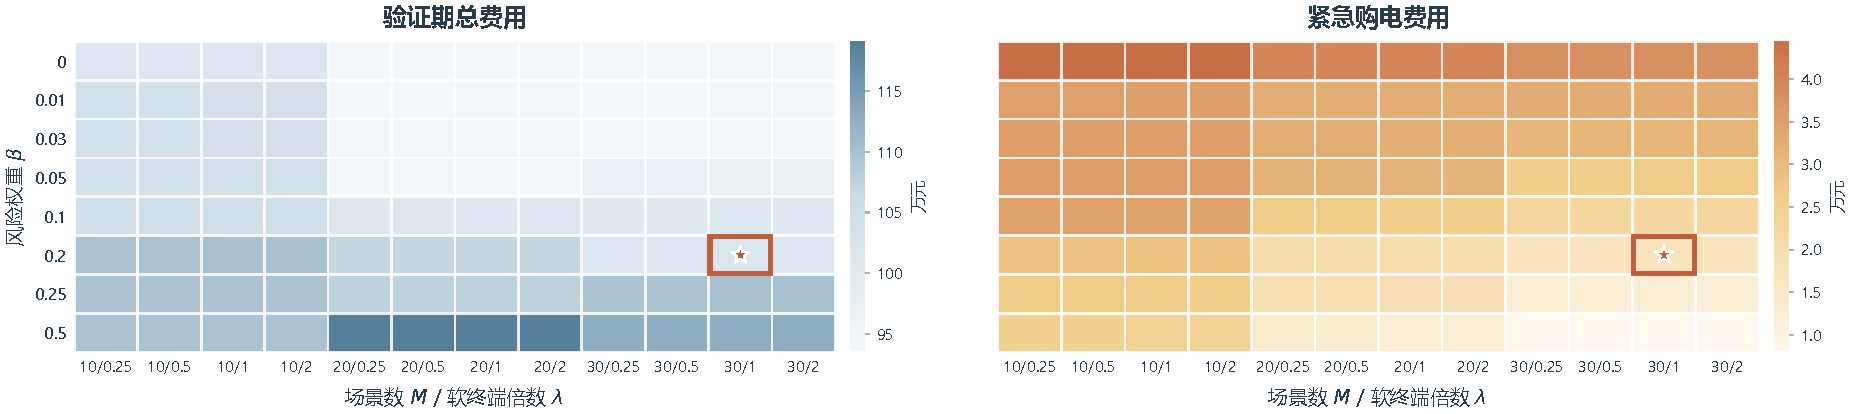
\includegraphics[width=0.95\textwidth]
    {../All_Code/Q2_yy/Results/Pictures/fig_q2_cvar_frontier.pdf}
    \caption{验证期候选参数的费用与风险分布}
    \label{fig:q2_cvar_frontier}
\end{figure}

候选参数在总费用与紧急购电风险之间存在明显取舍：部分组合总费用更低，但紧急购电费用超过基准，不满足筛选条件。
图中红色星号标记满足限制且评价指标最小的组合。最终得到
\begin{equation}
    M^{\ast}=30,\qquad
    \beta^{\ast}=0.20,\qquad
    \lambda^{\ast}=1,\qquad
    \kappa_2^{\ast}
    =\lambda^{\ast}\kappa_{2,\mathrm{base}}
    =0.531667
    \label{eq:q2_optimal_parameters}
\end{equation}
该组合验证期总费用为 \(1016195.38\) 元，紧急购电费用为 \(16517.07\) 元，期末储电量 \(6000\,\mathrm{kWh}\)；参数于1月31日确定，此后在报告期滚动求解中保持不变。
\subsection{求解结果与分析}

\subsubsection{指定日期购电结果}

根据正式报告期的滚动求解结果，本文选取题目指定的四个日期进行分析。
表~\ref{tab:q2_selected_purchase} 给出各指定时段的计划购电量、全天计划购电量与购电费用；其中购电费用不含实际运行中产生的紧急购电费用。

\definecolor{headerblue}{RGB}{174,205,230}
\definecolor{datablue}{RGB}{229,241,250}

\begin{table}[H]
    \centering
    \caption{指定日期计划购电结果}
    \label{tab:q2_selected_purchase}
    \small
    \setlength{\tabcolsep}{6pt}
    \renewcommand{\arraystretch}{1.22}

    \resizebox{0.92\textwidth}{!}{%
    \begin{tabular}{|c|c|c|c|c|}
        \hline
        \rowcolor{headerblue}
        \textbf{指标}
        & \textbf{2025年3月20日}
        & \textbf{2025年6月21日}
        & \textbf{2025年9月23日}
        & \textbf{2025年12月21日} \\
        \hline
        \(10{:}00\) 至 \(10{:}10\) & 0.00 & 0.00 & 0.00 & 0.00 \\
        \hline
        \(12{:}00\) 至 \(12{:}10\) & 709.43 & 0.00 & 535.02 & 968.20 \\
        \hline
        \(14{:}00\) 至 \(14{:}10\) & 0.00 & 0.00 & 0.00 & 0.00 \\
        \hline
        \(16{:}00\) 至 \(16{:}10\) & 523.93 & 279.17 & 591.29 & 853.60 \\
        \hline
        \(18{:}00\) 至 \(18{:}10\) & 712.75 & 131.28 & 840.90 & 719.97 \\
        \hline
        \(20{:}00\) 至 \(20{:}10\) & 0.00 & 0.00 & 21.61 & 0.00 \\
        \hline
        \textbf{全天计划购电量}
        & \cellcolor{datablue}\textbf{71479.42}
        & \cellcolor{datablue}\textbf{42324.35}
        & \cellcolor{datablue}\textbf{76040.75}
        & \cellcolor{datablue}\textbf{100109.36} \\
        \hline
        \textbf{全天计划购电费}
        & \cellcolor{datablue}\textbf{43233.44}
        & \cellcolor{datablue}\textbf{24565.93}
        & \cellcolor{datablue}\textbf{48103.80}
        & \cellcolor{datablue}\textbf{64432.16} \\
        \hline
    \end{tabular}%
    }

    \par\smallskip
    {\footnotesize
    注：指定时段购电量与全天计划购电量的单位为
    \(\mathrm{kWh}\)，购电费用的单位为元。
    }
\end{table}

四个指定日期中，6月21日的计划购电量和费用最低，12月21日最高，体现了季节性供需差异。
各日期在 \(10{:}00\) 和 \(14{:}00\) 附近均无须购电，而傍晚光伏出力下降后，外网购电需求普遍增加。
真实供需与日前预测产生的偏差则由紧急购电补足。

\begin{table}[H]
    \centering
    \caption{指定日期紧急购电结果}
    \label{tab:q2_emergency_purchase}
    \scriptsize
    \setlength{\tabcolsep}{3pt}
    \renewcommand{\arraystretch}{1.15}

    \begin{tabularx}{\textwidth}
    {|>{\centering\arraybackslash}p{0.045\textwidth}
     |>{\centering\arraybackslash}X
     |>{\centering\arraybackslash}X
     |>{\centering\arraybackslash}X
     |>{\centering\arraybackslash}X|}
        \hline
        \rowcolor{headerblue}
        \textbf{序号}
        & \textbf{2025年3月20日}
        & \textbf{2025年6月21日}
        & \textbf{2025年9月23日}
        & \textbf{2025年12月21日} \\
        \hline

        1
        & \(0{:}20\) 至 \(0{:}30\) / 25.513
        & \(1{:}20\) 至 \(1{:}30\) / 5.806
        & \(2{:}10\) 至 \(2{:}20\) / 5.785
        & \(1{:}10\) 至 \(1{:}20\) / 4.035 \\
        \hline

        2
        & \(1{:}00\) 至 \(1{:}30\) / 70.576
        & \(3{:}00\) 至 \(3{:}30\) / 38.256
        & \(5{:}00\) 至 \(5{:}10\) / 4.611
        & \(3{:}30\) 至 \(3{:}50\) / 46.272 \\
        \hline

        3
        & \(3{:}10\) 至 \(3{:}30\) / 36.112
        & \(3{:}50\) 至 \(4{:}10\) / 29.296
        & \(10{:}40\) 至 \(10{:}50\) / 12.817
        & \(10{:}30\) 至 \(11{:}30\) / 343.028 \\
        \hline

        4
        & \(3{:}40\) 至 \(4{:}00\) / 20.465
        & \(5{:}00\) 至 \(5{:}10\) / 9.869
        & \(14{:}30\) 至 \(15{:}10\) / 80.996
        & \(12{:}40\) 至 \(13{:}00\) / 49.292 \\
        \hline

        5
        & \(4{:}50\) 至 \(5{:}20\) / 29.221
        & \(5{:}20\) 至 \(5{:}40\) / 24.229
        & \(22{:}20\) 至 \(22{:}30\) / 26.117
        & \(16{:}20\) 至 \(16{:}30\) / 0.300 \\
        \hline

        6
        & \(6{:}40\) 至 \(7{:}00\) / 14.940
        & \(5{:}50\) 至 \(6{:}20\) / 43.451
        & --
        & \(16{:}50\) 至 \(17{:}00\) / 0.808 \\
        \hline

        7
        & \(9{:}00\) 至 \(9{:}10\) / 4.823
        & \(8{:}30\) 至 \(8{:}40\) / 10.352
        & --
        & \(17{:}20\) 至 \(17{:}30\) / 14.512 \\
        \hline

        8
        & \(10{:}50\) 至 \(11{:}30\) / 101.086
        & \(9{:}00\) 至 \(9{:}10\) / 21.105
        & --
        & \(18{:}10\) 至 \(19{:}10\) / 73.217 \\
        \hline

        9
        & \(15{:}20\) 至 \(16{:}20\) / 174.705
        & \(18{:}40\) 至 \(18{:}50\) / 9.759
        & --
        & \(19{:}20\) 至 \(19{:}30\) / 2.285 \\
        \hline

        10
        & \(16{:}30\) 至 \(17{:}20\) / 75.633
        & --
        & --
        & \(19{:}40\) 至 \(20{:}00\) / 52.077 \\
        \hline

        11
        & \(18{:}10\) 至 \(18{:}20\) / 2.788
        & --
        & --
        & \(20{:}30\) 至 \(20{:}40\) / 0.880 \\
        \hline

        12
        & \(18{:}40\) 至 \(19{:}10\) / 29.317
        & --
        & --
        & \(21{:}50\) 至 \(22{:}00\) / 7.527 \\
        \hline

        13
        & \(20{:}00\) 至 \(20{:}20\) / 46.283
        & --
        & --
        & \(23{:}30\) 至 \(23{:}40\) / 5.441 \\
        \hline

        14
        & \(23{:}30\) 至 \(23{:}40\) / 14.212
        & --
        & --
        & -- \\
        \hline

        \rowcolor{datablue}
        \textbf{合计}
        & \textbf{645.674}
        & \textbf{192.123}
        & \textbf{130.325}
        & \textbf{599.675} \\
        \hline
    \end{tabularx}

    \par\smallskip
    {\footnotesize
    注：各单元格依次表示紧急购电时段和购电量，购电量单位为
    \(\mathrm{kWh}\)，相邻的十分钟紧急购电时段已合并。
    }
\end{table}
表~\ref{tab:q2_emergency_purchase} 将相邻的紧急购电时段合并为连续区间，并汇总相应购电量。
3月20日的紧急购电量最高，为
\(645.674\,\mathrm{kWh}\)，9月23日最低，为
\(130.325\,\mathrm{kWh}\)。
12月21日的紧急购电主要集中在
\(10{:}30\) 至 \(11{:}30\)，该时段购电量占当日紧急购电量的一半以上。
计入紧急购电后，6月21日的总费用最低，为
\(25216.26\)元，12月21日最高，为
\(66729.15\)元。

为进一步说明日前计划在真实数据到达后的执行过程，本文选取
2025年6月1日作为代表日，将十分钟结算结果按小时汇总，结果见附录~\ref{app:q2_typical_day}。
实际需求低于计划时，未提取电量仍需计费；实际需求超过可用电量时则通过紧急购电补足。
该日计划购电量为 \(68.9\,\mathrm{MWh}\)，紧急购电量为
\(8.4\,\mathrm{MWh}\)，其中11时的缺口最为显著。

\subsubsection{指定日期储能调度结果}

四个指定日期的分时段储能充放电量见附录~\ref{app:q2_typical_day}。
储能主要在凌晨和光伏富余时段充电，并在
\(16{:}00\) 至 \(20{:}00\) 集中放电。
6月21日的充放电规模最小，12月21日最大，体现了不同季节供需条件下调度策略的差异。
同一四小时区间内出现充电和放电，是由不同十分钟时段的操作汇总所致，并非同时充放电。

\subsubsection{报告期费用与供需偏差分析}

2025年2月1日至12月31日共完成334天滚动调度。
报告期计划购电量为
\(22707.619\,\mathrm{MWh}\)，计划购电费用为
\(13885012.62\)元。
实际运行中产生紧急购电
\(217.628\,\mathrm{MWh}\)，对应费用为
\(823950.87\)元。
最终总购电费用为
\(14708963.49\)元，其中紧急购电费用占
\(5.602\%\)。

计划购电中实际提取
\(21172.617\,\mathrm{MWh}\)，其余
\(1535.002\,\mathrm{MWh}\) 未被提取，但仍按照全天计划计费。
报告期储能充电量和放电量分别为
\(7066.246\,\mathrm{MWh}\) 和
\(5723.660\,\mathrm{MWh}\)，二者比例与
\(81\%\) 的往返效率一致。

为观察供电不足和光伏过剩的季节分布，将紧急购电量与弃光量按月汇总，结果如图~\ref{fig:q2_monthly_emergency_curtailment} 所示。

\begin{figure}[H]
    \centering
    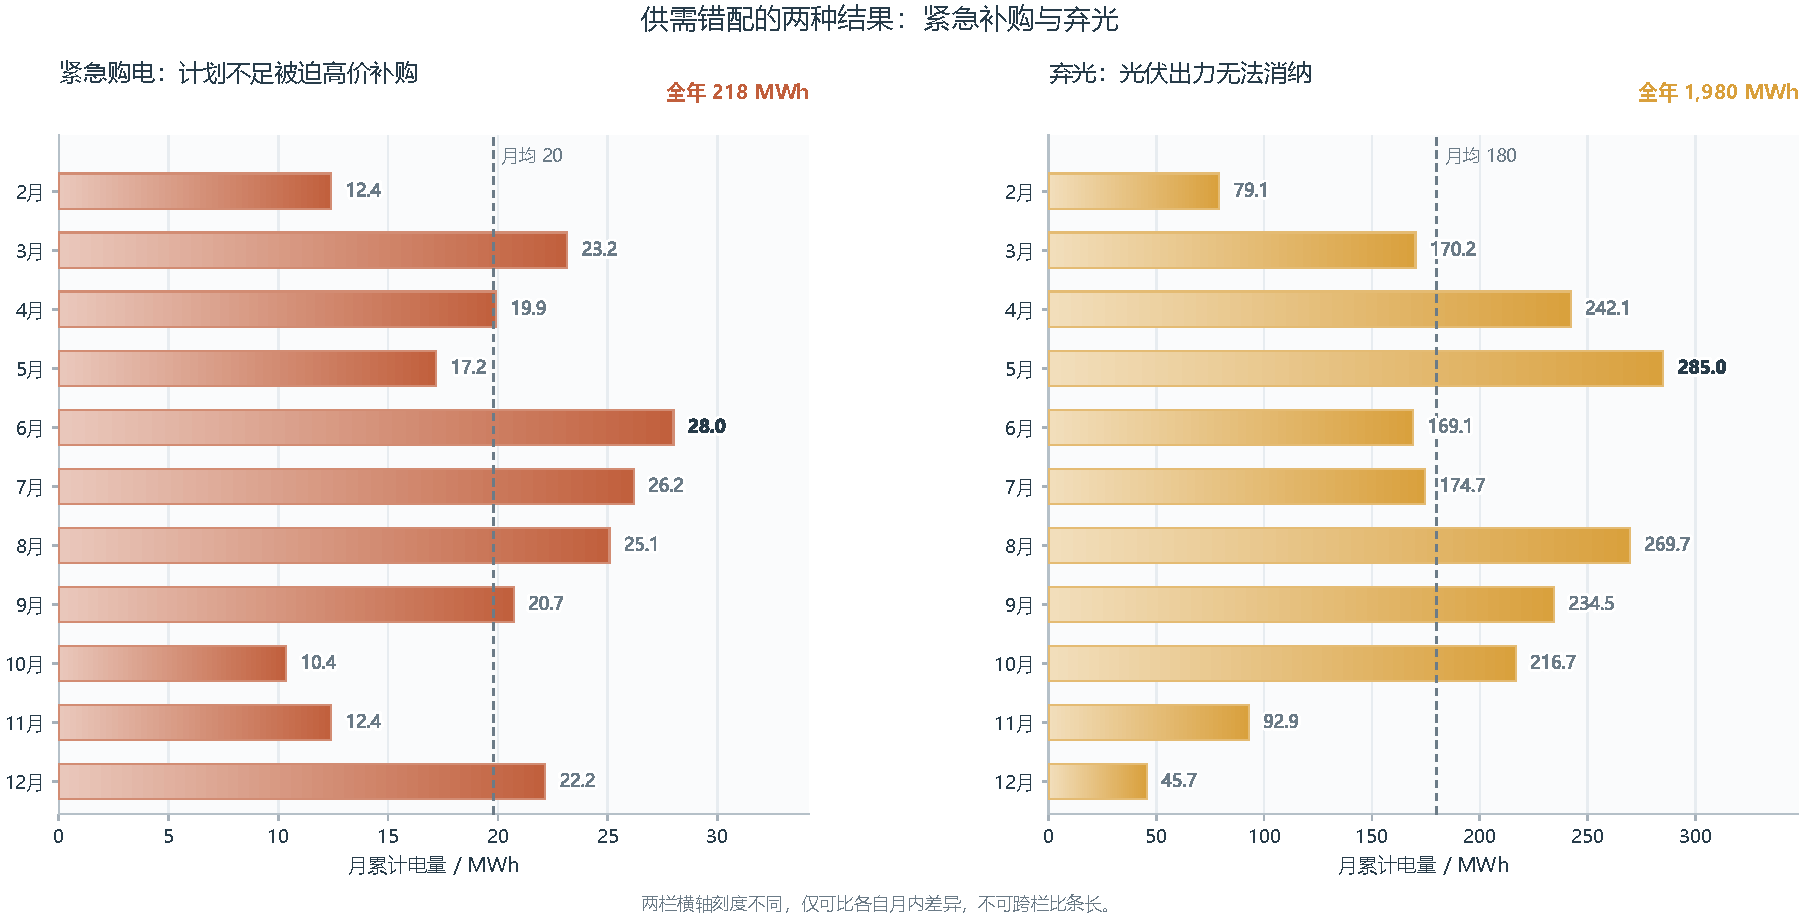
\includegraphics[width=0.8\textwidth]
    {../All_Code/Q2_yy/Results/Pictures/fig_q2_emergency_curtailment.pdf}
    \caption{报告期紧急购电量与弃光量的月度分布}
    \label{fig:q2_monthly_emergency_curtailment}
\end{figure}

紧急购电量在6月达到最高值
\(28.0\,\mathrm{MWh}\)，7月和8月也处于较高水平，说明夏季实际净负荷偏离日前计划的情况更为突出。
弃光量在5月达到最高值
\(285.0\,\mathrm{MWh}\)，并在4月、8月和9月保持较高水平，表明光伏富余具有明显的季节性。
图中数值表示月累计电量，颜色深浅仅用于比较同一指标在不同月份的相对大小。

报告期累计弃光量为
\(1979.773\,\mathrm{MWh}\)。
此外，固定日前放电计划在275个调度日产生
\(128.696\,\mathrm{MWh}\) 的供给过剩弃电。
未提取计划电量、弃光量和供给过剩弃电分别反映计划过量、光伏过剩和固定放电过剩，三者不能合并统计。

\subsection{模型检验}

本文对预测因果性、约束满足情况和结果文件进行独立检验。
预测与场景生成均未使用决策时刻之后的信息，电量平衡和储能状态转移的最大残差分别为
\(2.27\times10^{-13}\,\mathrm{kWh}\) 和
\(9.09\times10^{-13}\,\mathrm{kWh}\)，各项运行边界均得到满足。
费用复算结果与程序输出一致，表明模型求解与结果导出具有可靠性。
完整检验过程及模型局限见附录~\ref{app:q2_validation}。





